\begin{frame}
    \centering
    \Large\textbf{Addressing the Impossible Trinity of Modeling}
\end{frame}

\begin{frame}{\small How does \textbf{physics-infused} ROMs (PIROMs) \textbf{solve the ITM} in small-data regimes?}
    \begin{center}
        {\small \textbf{Let us consider the following example}:}\\
        {\small Hypersonic Thermal Protection Systems (TPS)}
    \end{center}
    \begin{figure}
        \centering
        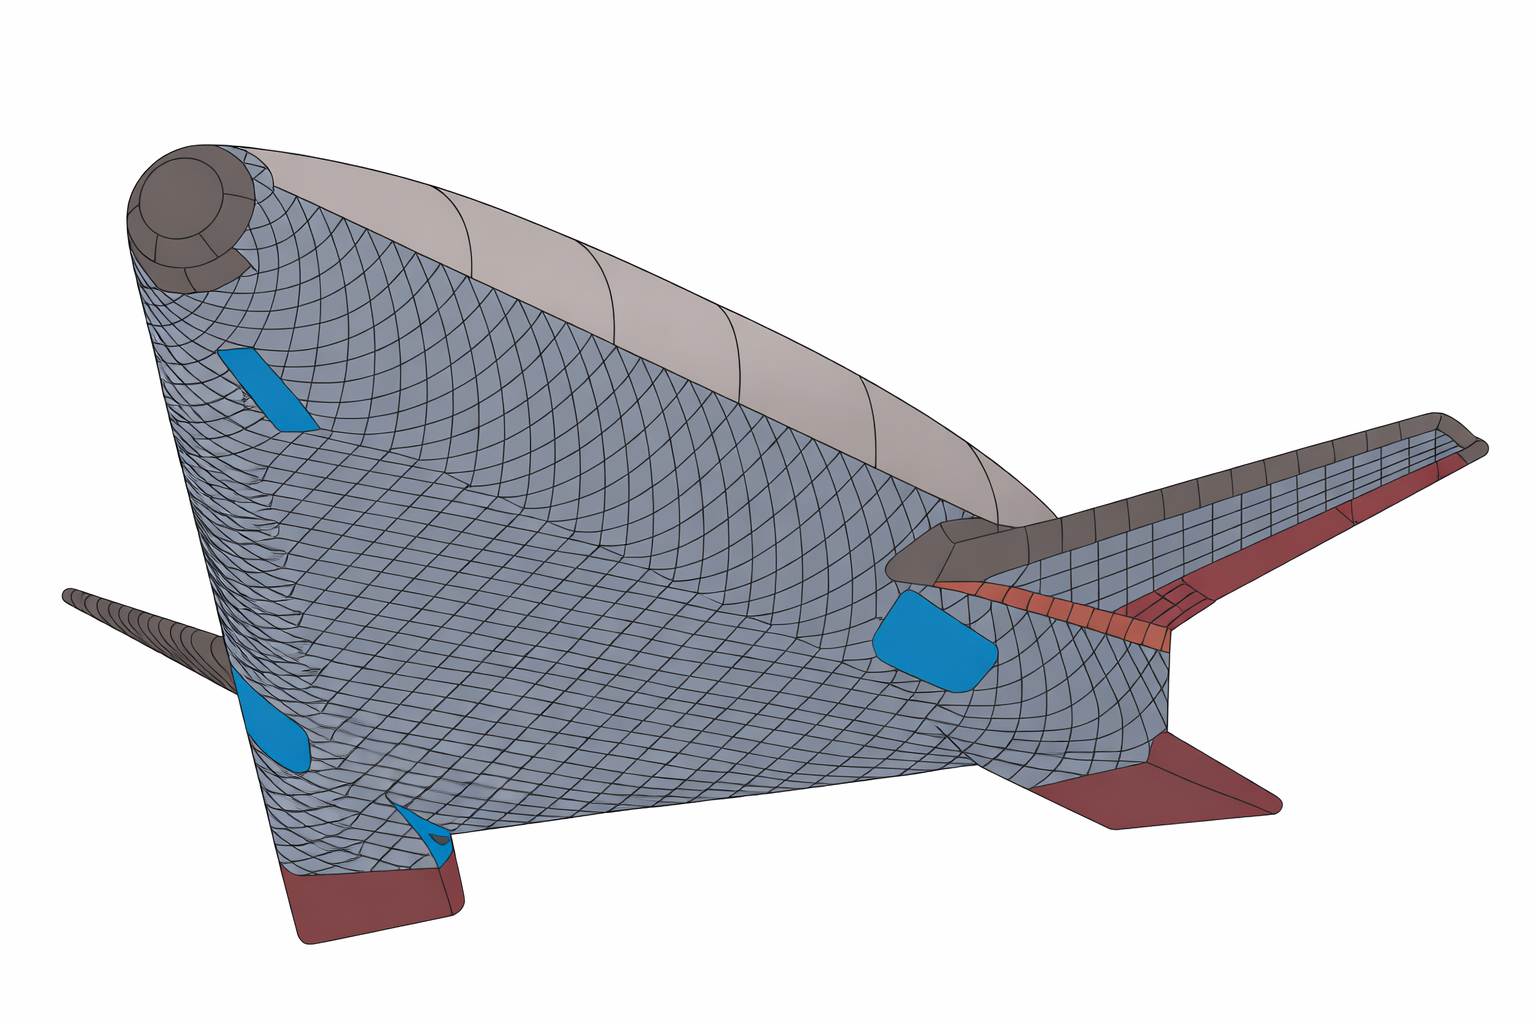
\includegraphics[width=0.4\textwidth]{../figs/tps/tps_vehicle.png}
    \end{figure}
\end{frame}

\begin{frame}{\small We start from the \textbf{FOM}, and reduce its \textbf{complexity via coarse-graining},}
    \footnotesize
    \begin{columns}
        \begin{column}{0.55\textwidth}
            \begin{figure}
                \centering
                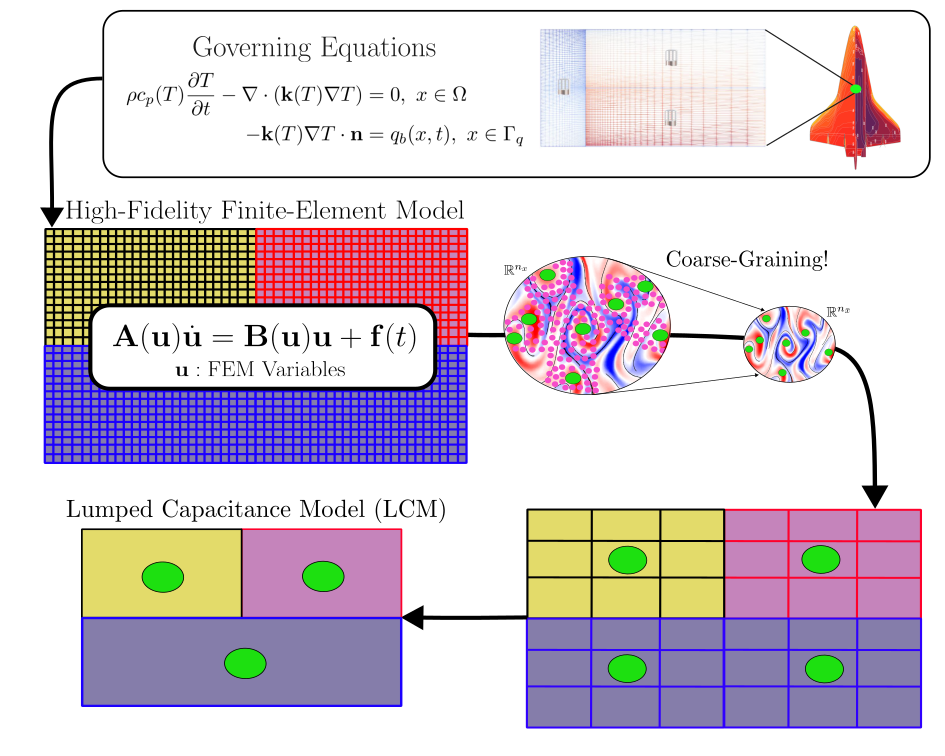
\includegraphics[width=0.85\textwidth]{../figs/pirom/coarse_graining_tps_left_4.png}
            \end{figure}
        \end{column}
        \hspace*{-0.3in}
        \begin{column}{0.55\textwidth}
                \begin{figure}
                    \centering
                    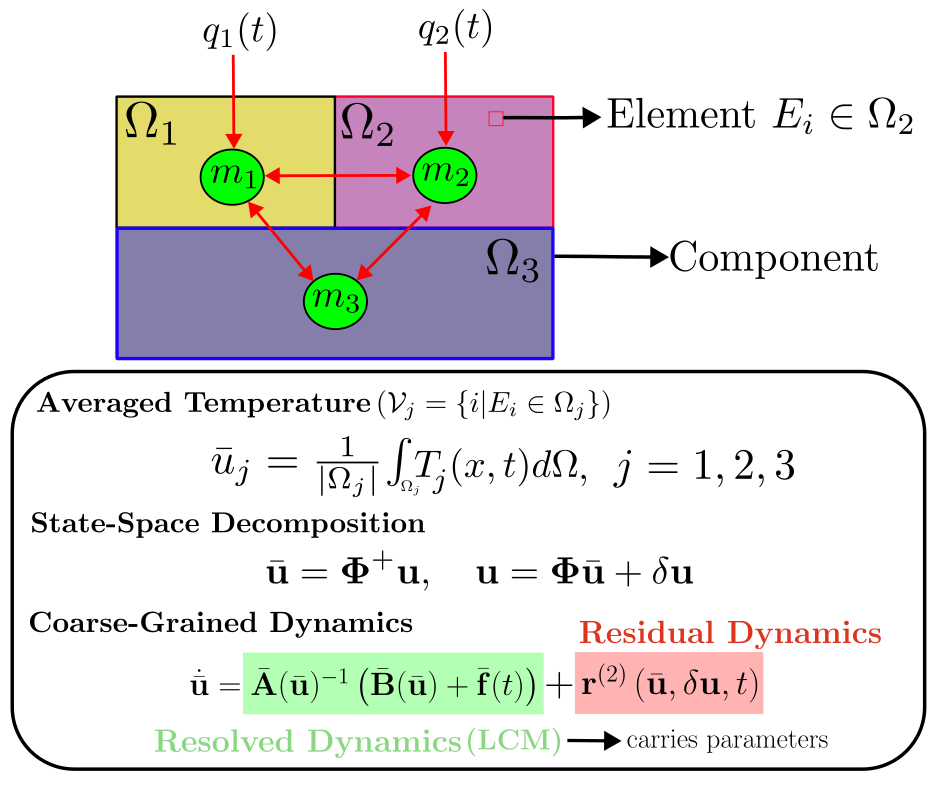
\includegraphics[width=0.95\textwidth]{../figs/pirom/coarse_grained_variables_tps_6.png}
                \end{figure}
        \end{column}
    \end{columns}
\end{frame}

\begin{frame}{\small Next, we employ the Mori-Zwanzig formalism for \textbf{physics infusion},}
    \footnotesize
    \begin{equation*}
        \text{Projected GLE}:\quad \underbrace{\frac{\partial}{\partial t} \cP e^{t\cL}\bvu}_{\text{Observable Dynamics}} = \underbrace{\cP e^{t\cL}\cP\cL\bvu}_{\text{Markovian}} + \cP\underbrace{\int_0^t e^{(t-s)\cL}\cP\cL e^{s\cQ\cL}\cQ\cL\bvu ds}_{\text{Non-Markovian}}+ \cP\underbrace{e^{t\cQ\cL}\cQ\cL\bvu}_{\text{Noise}}
    \end{equation*}
    \begin{columns}
        \begin{column}{0.3\textwidth}
            \centering
            \textbf{Markovian}
            \begin{figure}
                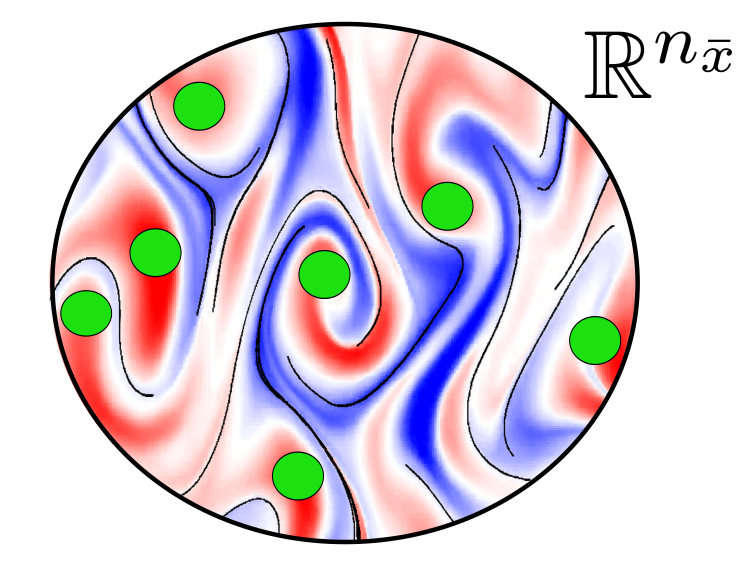
\includegraphics[width=0.9\textwidth]{../figs/pirom/coarse_variables.png}
            \end{figure}
            {\small (known dynamics)}
        \end{column}
        \begin{column}{0.3\textwidth}
            \centering
            \textbf{Non-Markovian}
            \begin{figure}
                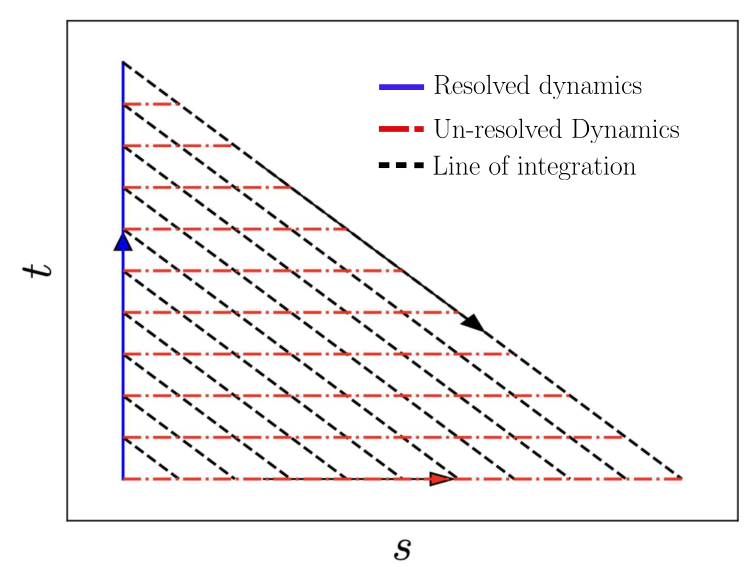
\includegraphics[width=0.9\textwidth]{../figs/pirom/memory.png}{\tiny [1]}
            \end{figure}
            {\small\textcolor{red}{(unknown dynamics)}}
        \end{column}
        \begin{column}{0.3\textwidth}
            \centering
            \textbf{Noise}
            \begin{figure}
                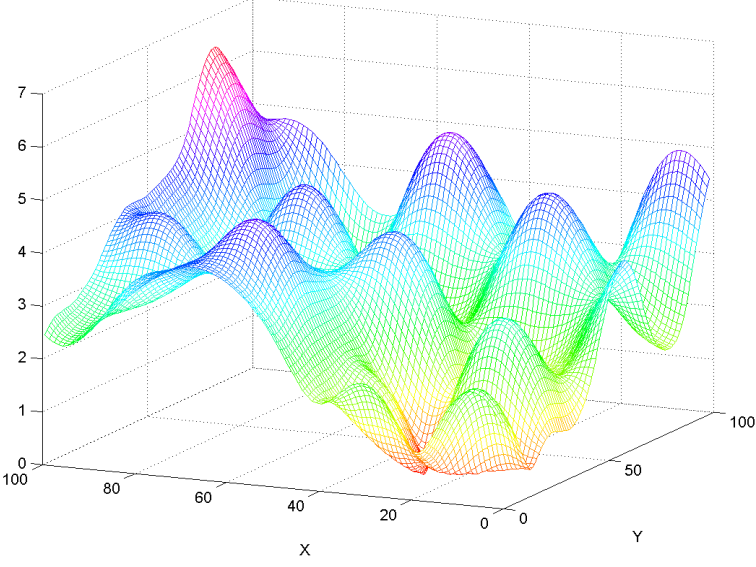
\includegraphics[width=0.9\textwidth]{../figs/pirom/noise.png}
            \end{figure}
            {\small\textcolor{black}{(orthogonal to $\cP$)}}
        \end{column}
    \end{columns}
    \begin{center}
        {\tiny GLE: Generalized Langevin Equation, $\cL$: Liouville operator, PGLE: Projected GLE}
    \end{center}
\end{frame}

\begin{frame}{\small Next, we employ the Mori-Zwanzig (MZ) formalism for \textbf{physics infusion},}
    \footnotesize
    \begin{columns}
        \begin{column}{0.5\textwidth}
            \begin{graybox}{Memory Kernel Parametrization}
                Define the memory kernel,
                \begin{equation*}
                    \vkappa(\bvu,t,s) = \cP e^{(t-s)\cL}\cP\cL e^{s\cQ\cL}\cQ\cL\bvu
                \end{equation*}
                Parametrize the \textbf{memory kernel},
                \begin{equation*}
                    \vkappa(\bvu,t,s;\redvTheta) \approx \sum_{j=1}^{m} \cK_j(t,s,\bvu;\redvTheta)\phi_j(s,\bvu;\redvTheta)
                \end{equation*}
                For \textbf{TPS problem}, design $\cK_j$ and $\phi_j$ as,
                \begin{align*}
                    \cK_j(t,s,\bvu;\redvTheta) &= e^{-\textcolor{red}{\lambda_j}(t-s)}\Rightarrow\text{{\tiny \textbf{exponential decay!}}}\\
                    \phi_j(s,\bvu;\redvTheta) &= \textcolor{red}{\vp_j}\left(\textcolor{red}{\vq_j}^\top\bar{\vu}(s) + \textcolor{red}{\vr_j}^\top\underbrace{\bar{\vf}(s)}_{\text{external forcing}} \right)
                \end{align*}
            \end{graybox}
        \end{column}
        \hspace*{-0.1in}
        \begin{column}{0.55\textwidth}
            \begin{graybox}{Markovian Reformulation}
                Define the \textbf{memory variables} as,
                \begin{equation*}
                    \beta_j(t) = \int_0^t e^{-\textcolor{red}{\lambda_j}(t-s)} \left(\textcolor{red}{\vq_j}^\top\bar{\vu}(s) + \textcolor{red}{\vr_j}^\top\bar{\vf}(s)\right) ds
                \end{equation*}
                so that the \textbf{hidden dynamics} are,
                \begin{equation*}
                    \dot{\beta}_j = \textcolor{red}{\lambda_j}\beta_j + \textcolor{red}{\vq_j}^\top\bar{\vu} + \textcolor{red}{\vr_j}^\top\bar{\vf},\:\: j=1,\dots,m
                \end{equation*}
                Thus, \textbf{the PIROM may be written as},
                \begin{align*}
                    \dot{\bvu} &= \underbrace{\cP e^{t\cL}\cP\cL\bvu}_{\text{\textbf{LCM dynamics!}}} + \sum_{j=1}^{m}\textcolor{red}{\vp_j}\beta_j\\
                    \dot{\beta}_j &= \textcolor{red}{\lambda_j}\beta_j + \textcolor{red}{\vq_j}^\top\bar{\vu} + \textcolor{red}{\vr_j}^\top\bar{\vf}\\
                    \vz &= \textcolor{red}{\vD_{\bar{u}}}\bvu + \textcolor{red}{\vD_{\beta}}\boldsymbol{\beta}
                \end{align*}
                $\redvTheta = \left\{\textcolor{red}{\vP,\vQ,\vLambda,\vR,\vD_{\bar{u}},\vD_{\beta}}\right\}$ \textcolor{red}{optimize parameters!}
            \end{graybox}
        \end{column}
    \end{columns}
\end{frame}

\begin{frame}{\small \textbf{Compare the PIROM} to state-of-the-art SCiML methods,}
    \footnotesize
    \begin{figure}
        \centering
        
\includegraphics[width=1.05\textwidth]{../figs/pirom/performance_5.png}
    \end{figure}
    \begin{center}
        {\tiny NODE: neural ordinary differential equations, OpInf: operator inference, NRMSE: normalized root mean square error}
    \end{center}
\end{frame}

\begin{frame}{\small Is the Impossible Trinity of Modeling \textbf{solved}?}
    \footnotesize
    \begin{columns}
        \begin{column}{0.3\textwidth}
            \vspace*{0.3in}
            \centering
            \begin{figure}
                \centering
                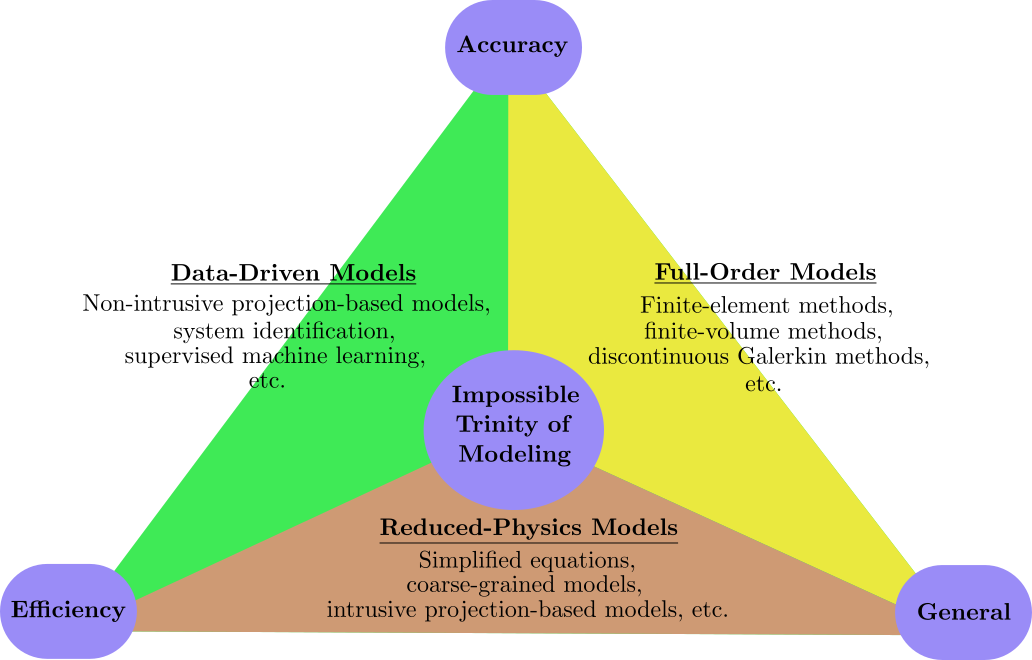
\includegraphics[width=0.9\textwidth]{../figs/introduction/itm.png}
            \end{figure}
        \end{column}
        \begin{column}{0.8\textwidth}
            \centering
            \begin{itemize}
                \item \textbf{Accuracy}: comparable to FOMs (NRMSE $<1\%$),
                \item \textbf{Efficiency}: two-to-three orders of magnitude faster than FOMs,
                \item \colorbox{green!30}{\textbf{Generalizability}}:
                \begin{itemize}
                    \item \colorbox{green!30}{\textbf{Dimensions}: un-seen loading conditions},
                    \item \colorbox{green!30}{\textbf{Physics}: un-seen material properties} 
                \end{itemize}
                \item \textbf{What about training efficiency?}
                \begin{itemize}
                    \item \textbf{Overhead} is \colorbox{red!30}{$\approx$ 4 hrs in 3 CPUs} (similar to NODE),
                    \item therefore, we need to explore \colorbox{red!30}{other training approaches!}
                \end{itemize}
            \end{itemize}
        \end{column}
    \end{columns}
    \begin{tikzpicture}[remember picture, overlay]
        \node[anchor=north west, xshift=1.86cm, yshift=-3.4cm] at (current page.north west) {
\includegraphics[width=0.05\textwidth]{../figs/pirom/checkmark.png}};
    \end{tikzpicture}
    \begin{tikzpicture}[remember picture, overlay]
        \node[anchor=north west, xshift=0.22cm, yshift=-5.5cm] at (current page.north west) {
\includegraphics[width=0.05\textwidth]{../figs/pirom/checkmark.png}};
    \end{tikzpicture}
    \begin{tikzpicture}[remember picture, overlay]
        \node[anchor=north west, xshift=3.52cm, yshift=-5.5cm] at (current page.north west) {
\includegraphics[width=0.05\textwidth]{../figs/pirom/checkmark.png}};
    \end{tikzpicture}
\end{frame}